\section{Citation Analysis} \label{sec:citation-analysis}

A citation establishes a connection from one document to another, creating a relationship between the document that cites and the one that is cited. The study of these relationships constitutes citation analysis, a central element of bibliometrics \cite{SmithCitationAnalysis1981}.

Citation analysis offers a valuable method for assessing the relevance of scientific papers. It can be used to identify related works, track the evolution of research trends, and understand the structure of a knowledge field \cite{Marshakova-ShaikevichSystemDocument1973}. This section provides an overview of the different approaches to citation analysis, with a particular focus on bibliographic coupling and co-citation analysis. The section also explores how citation analysis can enhance paper recommender systems.


\subsubsection*{Citation Count as a Measure of Relevance}

A simple approach to utilizing citation information for relevance is to take into account the paper's citation count, that is, the number of times a paper has been cited, as a marker of its relevance.
However, Smith \cite{SmithCitationAnalysis1981} points out that this method can be short-sighted as the influence of a paper may not necessarily align with its citation count, since not all citations carry equal significance. Some citations are given out of respect or convention, without the cited papers significantly affecting the citing one. Thus, while citation count offers an insight into a work's impact, it shouldn't stand as the sole metric for determining relevance \cite{SmithCitationAnalysis1981}.

Additionally, Marshakova-Shaikevich \cite{Marshakova-ShaikevichSystemDocument1973} emphasizes the need for a comprehensive review of all references in documents related to that field, which goes beyond a mere citation count.
Finally, citation counts lack sensitivity to specific reference or query documents, rendering them as static for all researchers, with no option for personalization.


\subsubsection*{Using Connections Between Papers}

A refined approach beyond simply counting citations involves considering connections between papers.
Related papers can be identified by examining the direct connections between \emph{citing} and \emph{cited} papers. Cited papers, or \emph{outgoing links}, are all references found in a paper's bibliography. Conversely, citing papers, or \emph{incoming links}, are all papers that cite the paper of interest.

However, direct connections aren't always the most indicative of relatedness.
Very popular papers are commonly cited out of convention, without a strong link to the citing paper's topic.
Additionally, some researchers might over-cite their own works or those of close colleagues to boost their citation count, creating a false impression of relatedness.

To address these problems, researchers have turned to methods like bibliographic coupling, co-citation analysis, and citation context analysis, which use indirect connections between papers to reveal associations between works that might not be apparent from direct citations \cite{SmithCitationAnalysis1981}. These methods help create a citation network, a set of documents related through citations, which can be represented as a directed graph. As noted by Marshakova-Shaikevich \cite{Marshakova-ShaikevichSystemDocument1973}, this graph can be used to identify clusters of closely related documents, track the progression of ideas and research trends, and understand the structure of a knowledge field.


\subsection{Bibliographic Coupling \& Co-Citation Analysis} \label{sec:bibliographic-coupling-co-citation-analysis}

Throughout this thesis, we distinguish between the terms \emph{citation} and \emph{reference}. Echoing Breitinger \cite{BreitingerAcademicLiterature2023}, we define \emph{citations} as the in-text markers pointing to other research papers, while \emph{references} refer to the list of cited papers at the end of a research paper, commonly termed the bibliography.

\emph{Bibliographic coupling} assesses the similarity between two articles by counting the references they share. The intuition is that if two articles cite many of the same sources, they likely address similar topics. The degree of similarity between two articles is directly proportional to the number of shared references. Moreover, this method can be employed for grouping papers, revealing the structure and evolution of scientific fields \cite{KesslerBibliographicCoupling1963,GippCitationProximity2009}.

Conversely, \emph{co-citation analysis} counts how often two articles are jointly cited in other papers. If two articles are frequently co-cited, it's assumed that they relate to each other. The strength of their relationship increases with the frequency of co-citations \cite{SmallCocitationScientific1973,GippCitationProximity2009}.

\begin{figure}[ht]
    \centering
    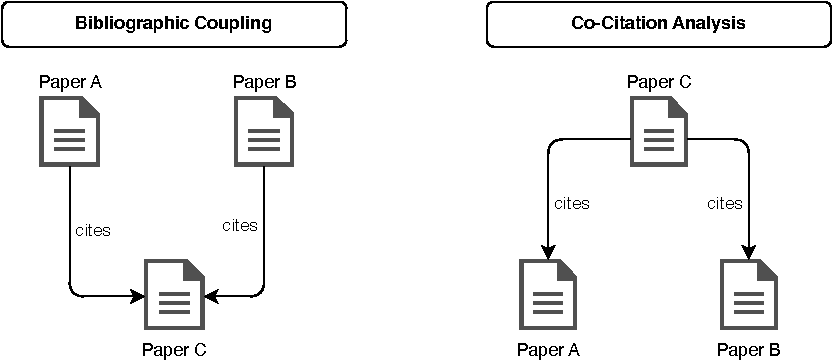
\includegraphics[width=0.8\textwidth]{diagrams/bibliographic_coupling_co_citation.pdf}
    \caption[Bibliographic Coupling vs. Co-Citation Analysis]{Bibliographic Coupling vs. Co-Citation Analysis, adapted from \cite{GippCitationProximity2009}.
        Left: Bibliographic coupling counts the number of shared references. Paper A and Paper B are connected by bibliographic coupling since they both cite the same Paper C. Right: Co-citation analysis counts the number of shared citing papers. Here, Paper A and Paper B are connected by co-citation analysis since they are both cited by Paper C.}
    \label{fig:bibliographic_coupling_co_citation}
\end{figure}

The difference between bibliographic coupling and co-citation analysis is visualized in \Cref{fig:bibliographic_coupling_co_citation}.
Numerically, the co-citation analysis score of an article is bounded by its total number of citations, while the bibliographic coupling score is bounded by its total number of references.
For instance, if paper A has 10 citations, the co-citation analysis score with any other paper B can be at most 10.
The maximum score is reached when all 10 citing papers of A also cite paper B.
Conversely, the maximum bibliographic coupling score is reached when the bibliography of paper A is a subset of the bibliography of paper B.


\subsubsection*{Comparison of Bibliographic Coupling and Co-Citation Analysis} \label{sec:comparison-of-bibliographic-coupling-and-co-citation-analysis}

When comparing the two approaches, Small \cite{SmallCocitationScientific1973} claims that co-citation analysis provides a more dynamic view of a field's intellectual structure, showing not only the relationships between works but also their relative importance and influence. Marshakova-Shaikevich \cite{Marshakova-ShaikevichSystemDocument1973} agrees, noting that bibliographic coupling is a static measure that doesn't consider the evolution of a document's relevance over time. She argues that co-citation analysis considers the future of a document through subsequent citations, whereas bibliographic coupling focuses on the document's past through its references.

However, both co-citation analysis and bibliographic coupling have their limitations. By definition, bibliographic coupling might miss relevant papers that don't share many common references with the paper of interest, while co-citation analysis may overlook papers that aren't frequently cited together with other papers. Additionally, bibliographic coupling tends to favor long documents that simply have more space to include references, while co-citation analysis favors older documents that have had more time to collect citations. Notably, both methods can be applied without full-text access, as they only require citation information or a bibliography. However, this implies that they ignore the \emph{location} of the citations within the text, which could provide valuable information about the relationship between the cited documents.

To address these shortcomings, \emph{location-aware} citation analysis methods have been developed. To identify the strength of the relationship between two citations, citation proximity can be measured at different levels of granularity including sentence, paragraph, and section levels \cite{TranEnrichingPubMed2009,LiuEffectsCocitation2011}.

Two popular approaches of location-aware citation analysis are \acl{CPA} and section-based bibliographic coupling.


\subsection{Citation Proximity Analysis} \label{sec:citation-proximity-analysis}

\ac{CPA} \cite{GippCitationProximity2009} is an improvement over traditional co-citation analysis, remedying some of its limitations. Whereas traditional co-citation analysis only takes into account the frequency of co-citations without considering their context or position within the text, \ac{CPA} introduces the concept of citation proximity, which refers to the textual distance between citations. It assumes that the closer two citations are to each other, the stronger their relationship is.

One practical application of \ac{CPA} is in paper recommendation, where it identifies related papers based on their \ac{CPA} score. Gipp et al. \cite{GippCitationProximity2009} suggest that \ac{CPA} could be combined with text mining algorithms to analyze the relationship between two references, thereby identifying agreeing or contradicting papers.

\subsubsection*{Citation Proximity Index} \label{sec:citation-proximity-index}

The \ac{CPI} quantifies the proximity score between two citations. Citations that are close to each other are assigned higher \ac{CPI} scores, while those further apart are assigned lower scores. The distance between citations is not determined by an absolute measure, like the number of characters between them, but is instead based on the document's structure. The highest \ac{CPI} is assigned to a citation pair within the same sentence (CPI=1), followed by the same paragraph (CPI=$\frac{1}{2}$), the same chapter (CPI=$\frac{1}{4}$), the same journal or book (CPI=$\frac{1}{8}$) and the same journal but different issues (CPI=$\frac{1}{16}$). The scoring is illustrated in \Cref{fig:citation-proximity-analysis} from Gipp et al. \cite{GippCitationProximity2009}.

\begin{figure}[ht]
    \centering
    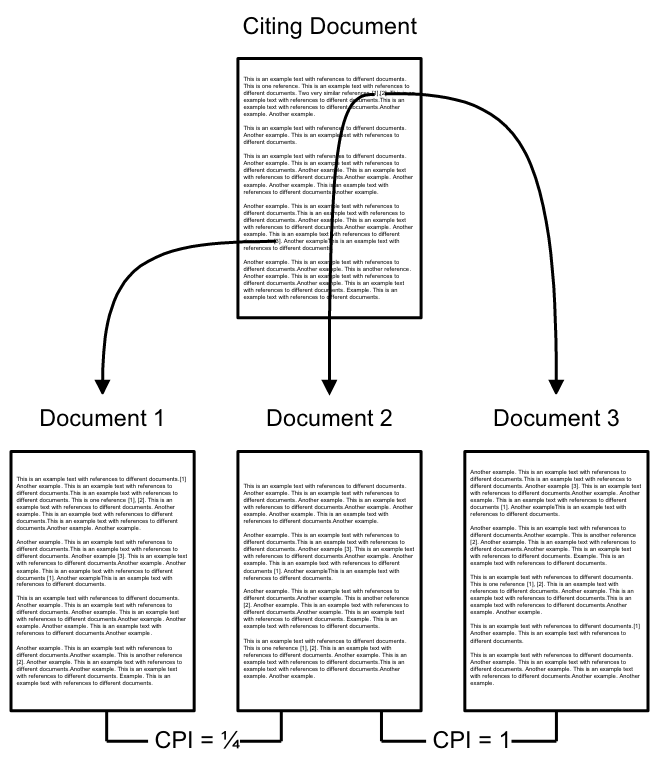
\includegraphics[width=0.5\textwidth]{screenshots/citation_proximity_analysis.png}
    \caption[\acl{CPA}]{\acl{CPA}, illustration from \cite{GippCitationProximity2009}.
        \ac{CPA} assigns positive \ac{CPI} values to document pairs with shared citing papers. The \ac{CPI} score depends on the proximity of the citations within the citing document.
        Documents 1 and 2 are co-cited within the same chapter but in different paragraphs of the citing document. Their \ac{CPI} score is $\frac{1}{4}$. Documents 2 and 3 are co-cited within the same sentence of the citing document; therefore, their \ac{CPI} score is $1$.}
    \label{fig:citation-proximity-analysis}
\end{figure}

In cases of multiple citation occurrences, e.g., once within the same sentence and once within the same paragraph, the highest \ac{CPI} is assigned to that citation pair. The \ac{CPI} between two \emph{papers} (instead of individual citations) is calculated by aggregating their individual \ac{CPI} scores across the entire corpus. Gipp et al. \cite{GippCitationProximity2009} found that using a weighted average yields the best results for aggregation.

\subsubsection*{Limitations of \acs{CPA}} \label{sec:limitations-of-cpa}

The authors assert that \ac{CPA} significantly outperforms traditional co-citation analysis for documents with either many references or few citations. However, \ac{CPA} has its limitations.
First, the authors note that the optimal weighting of the \ac{CPI} values might depend on the research field or research type.
Second, the \ac{CPI} scores heavily depend on the document's structure. Documents with longer sentences and sections contribute to higher \ac{CPI} values than those with shorter sentences and sections, as there is a higher probability of citations being within the same segment. Additionally, citation pairs with a large \emph{absolute} distance, e.g., between the first and last sentence of the same chapter, might be assigned a higher \ac{CPI} value than citation pairs with a small absolute distance, e.g., between the last and first sentence of consecutive chapters.

\subsubsection*{Alternative Proximity Measures} \label{sec:alternative-proximity-measures}

To address these shortcomings, Knoth and Khadka \cite{KnothCanWe2017} introduced alternative proximity measures: normalized \ac{CPA} (NCPA), inverse \ac{CPA} (ICPA), and squared inverse \ac{CPA} (SICPA). NCPA normalizes the proximity values based on the total number of co-citations within a document, whereas ICPA and SICPA assign higher weights to closer co-citations and decrease the weights continuously, rather than discretely, with increasing distance between co-citations. However, even these alternative proximity measures overlook the citation context.


\subsection{Section-based Bibliographic Coupling} \label{sec:section-based-bibliographic-coupling}

Section-based bibliographic coupling \cite{HabibSectionsbasedBibliographic2019} extends the concept of bibliographic coupling by considering the section of a document where a reference is cited. This approach recognizes that a citation in different sections of a paper might have different meanings or implications. For instance, a reference cited in the introduction might provide background information, while the same reference cited in the conclusion could support the author's argument. Habib et al. \cite{HabibSectionsbasedBibliographic2019} suggest that references from the \emph{Results} and \emph{Method} sections are more likely to be related to the paper's topic than references from the \emph{Introduction}, \emph{Conclusion}, and \emph{Related Work} sections, which might be more generic.

Similar to \ac{CPA}, section-based bibliographic coupling requires access to the full text of the document as it considers the location of citations. The methodology involves first identifying common references between a target paper and a candidate paper. Then, the citing patterns of the common references in different sections of the target and candidate papers are analyzed. Lastly, a section-based bibliographic coupling score is calculated, assigning different weights to citations based on their location within the paper. The Results and Method sections are assigned the largest weights, followed by the Introduction and Conclusion. The Related Work section is assigned the lowest weight \cite{HabibSectionsbasedBibliographic2019}.


\subsection{Applications in Paper Recommendation}

Citation analysis has found its way into various areas of research. For instance, Gipp et al. \cite{GippCitationbasedPlagiarism2014a} use citation analysis to spot plagiarism in academic papers. Unlike conventional character-based similarity measures, they analyze the citation placement within a document to identify semantically similar content, even without textual overlap. According to the authors, even when plagiarists disguise their work through translation, paraphrasing, or idea theft, they tend to retain the original citation pattern, making it a reliable indicator of plagiarism

However, the most prominent application of citation-based approaches is in scientific paper recommendation.
Sugiyama and Kan \cite{SugiyamaExploitingPotential2013} propose to identify "potential citation papers" that a researcher may not have cited in their work, but which are relevant to their research interests, to improve paper recommendation.
They use \ac{CF} techniques to identify these potential citation papers. The authors argue that different logical sections of a paper, such as the introduction, methodology, results, and conclusion, have different significance and could therefore be used to represent papers for recommendation in different ways. However, in contrast to section-based bibliographic coupling \cite{HabibSectionsbasedBibliographic2019}, their experiments show that assigning the largest weight to the conclusion section rather than the results and methodology sections leads to the best results.

Incorporating citation knowledge into recommender systems can also address the cold-start problem, as shown by Khadka et al. \cite{KhadkaCapturingExploiting2020}.
They use citation knowledge from direct and indirect citations such as co-citation analysis and bibliographic coupling to compute similarity scores between users and papers to generate personalized recommendations.
By mixing the citation-based approach with \ac{CF}, they emphasize that the citation component is essential for recommending \emph{recent} papers that lack user interaction and thus cannot be recommended by \ac{CF} alone.

Related to paper recommendation, Schwarzer et al. \cite{SchwarzerEvaluatingLinkbased2016} apply \ac{CPA} to the domain of Wikipedia articles to generate article recommendations by using links.
The authors argue that the links between Wikipedia articles play a similar role to citations in academic literature, providing a basis for similarity and thus for recommendations.
They demonstrate that citation-based methods are not only successful in the academic literature domain, but can also be effective in the distinct realm of Wikipedia.

On a meta-level, Ali et al. \cite{AliGraphbasedTaxonomy2020} present a comprehensive taxonomy to categorize citation recommendation models based on their underlying graph structures. The authors argue that graph structures are an appropriate basis for categorization because most citation recommendation models can be viewed as graph-based models. More specifically, these models often operate on graphs where nodes represent documents and edges represent relationships (e.g., citations or co-authorships).
The taxonomy distinguishes between four main categories: bibliographic coupling, co-citation, citation context, and hybrid models. This broader perspective on citation methods can facilitate a better understanding of different models and help with selecting suitable models for specific tasks.
